
%%%%%%%%%%%%%%%%%%%%%%%%%%%%%%%%%%%%%%%%%%%%%%%%%%%%%%%%%%%%%%%%%%%%%%%%%%%%%%%%
%
% Dark Matter Halos in the Early Universe
%
%%%%%%%%%%%%%%%%%%%%%%%%%%%%%%%%%%%%%%%%%%%%%%%%%%%%%%%%%%%%%%%%%%%%%%%%%%%%%%%%

\section{Dark Matter Halos in the Early Universe}
\label{sec:early_universe}

%%%%%%%%%%%%%%%%%%%%%%%%%%%%%%%%%%%%%%%%%%%%%%%%%%%%%%%%%%%%%%%%%%%%%%%%%%%%%%%%


Text goes here.




%~~~~~~~~~~~~~~~~~~~~~~~~~~~~~~~~~~~~~~~~~~~~~~~~~~~~~~~~~~~~~~~~~~~~~~~~~~~~~~~
\subsection{Halo Formation and Growth}
\label{subsec:early_universe--formation_and_growth}
%~~~~~~~~~~~~~~~~~~~~~~~~~~~~~~~~~~~~~~~~~~~~~~~~~~~~~~~~~~~~~~~~~~~~~~~~~~~~~~~


The attractive nature of gravity implies that regions of over-density become denser and regions of under-density become even more under-dense.  A perfectly smooth dark matter field would continue to stay smooth, as net forces would balance to zero.  However, small density perturbation generated during inflation in the otherwise smooth primordial DM field trigger the inexorable collapse of dark matter into over-dense regions known as dark matter halos \citep{1974ApJ...187..425P, 1986ApJ...304...15B}.

The non-linear evolution of the collapse of density fluctuations may be approximated to first order by the spherical ``top-hat'' perturbation \citep{1968ApJ...151..459S, 1970ApJ...162..815P, 1970AJ.....75...13P, 1972ApJ...176....1G}.  In this model, the perturbation is represented as an isolated, uniform sphere of dark matter.  The region outside the sphere is unperturbed and does not influence the evolution of the sphere.  This model affords an exact solution \citep[][and referencees therein]{1980lssu.book.....P, 1993ppc..book.....P, 1993sfu..book.....P}, but results in a collapse to infinite density.  However, growth of initially small density inhomogeneities may interrupt the collapse by a rapid relaxation to a finite density virial equilibrium \citep[][and references therein]{1999MNRAS.307..203S, 1998FCPh...19..157M}.

The definition of a halo arises from the contrast in density between a virialized over-dense region and the density of the rest of the universe.  For example, halos defined according to the spherical overdensity (SO) method are regions above a certain density threshold \citep{1998ApJ...495...80B}, either with respect to the critical density $\rho_{c} = 3 H^{2} / 8 \pi G$ or the background matter density $\rho_{b} = \Omega_{m} \rho_{c}$, where $\Omega_{m}$ is the matter density of the Universe.  The halo is then the region enclosed within a sphere with mean density $\Delta \rho_{c}$ or $\Delta \rho_{b}$, where $\Delta$ commonly ranges from $\sim 100$ to $\sim 500$ and is typically taken to be $\sim 200$.  The radius of the sphere is typically called the virial radius $\Rvir$, but may alternatively be denoted $R_{\Delta}$, where the specific choice of $\Delta$ is listed (e.g. $R_{200}$).

Dark matter halos form hierarchically \citep[e.g.,][and references therein]{2000MNRAS.319..168C, 2003AJ....126.1183C}.  Small halos form first from gravitational collapse and successively merge to form larger structures over time, which is often referred to as the ``bottom-up'' paradigm.  This leads to a characteristic mass of assembling halos at each redshift, which, at $z = 0$, are clusters with mass $\gtrsim 10^{14} \Msun$.  A typical halo undergoes a number of mergers throughout its evolution \citep[e.g.,][]{2003AJ....126.1183C, 2009ApJ...701.2002G, 2010MNRAS.406.2267F}.  Defining a major merger to have a mass ratio of $3:1$ or less and a minor merger to have a mass ratio of $10:1$ or less, a massive halo typically undergoes $\sim 4-5$ major mergers after $z \sim 3$, with minor mergers occurring even more frequently.  These mergers play a critical role in the mass assembly of a halo, and greatly influence the evolution of the hosted baryonic galaxy.




%~~~~~~~~~~~~~~~~~~~~~~~~~~~~~~~~~~~~~~~~~~~~~~~~~~~~~~~~~~~~~~~~~~~~~~~~~~~~~~~
\subsection{The Mass Function}
\label{subsec:early_universe--dark_matter_halos--mass}
%~~~~~~~~~~~~~~~~~~~~~~~~~~~~~~~~~~~~~~~~~~~~~~~~~~~~~~~~~~~~~~~~~~~~~~~~~~~~~~~


The number density of dark matter halos as a function of halo mass and redshift, often referred to simply as the mass function, is a key probe of cosmology.  The original formulation of \citet{1974ApJ...187..425P} is explored in more detail by a number of studies \citep[e.g.,][]{2002MNRAS.336..112M, 2006ApJ...646..881W}.  Here we follow the notation of \citet{2002MNRAS.336..112M}, where the number density of halos per unit comoving volume with mass in the interval $(M, M + \diff M)$ at redshift $z$ is given as
\begin{equation}
	n(M, z) \dd M = \sqrt{\frac{2}{\pi}} \frac{\bar{\rho_{0}}}{M} \frac{\diff \nu}{\diff M} \exp\left( -\frac{\nu^{2}}{2}\right) \dd M,
\end{equation}
where $\bar{\rho}_{0}$ is the current mean density of the universe, $\nu \equiv \delta_{c} / [D(z) \sigma(M)]$, $\delta_{c} \approx 1.69$, and the linear growth factor can be taken as $D(z) = g(z) / [g(0) (1 + z)]$ \citep{1992ARA&A..30..499C}, where
\begin{equation}
	g(z) \approx \frac{5}{2} \Omega_{m} \left[ \Omega_{m}^{4/7} - \Omega_{\Lambda} + (1 + \Omega_{m} / 2) (1 + \Omega_{\Lambda} / 70) \right]^{-1}.
\end{equation}
The density fractions are, as usual, functions of redshift:
\begin{equation}
	\Omega_{m} \equiv \Omega_{m}(z) = \frac{\Omega_{m,0} ( 1 + z )^{3}}{E^{2}(z)},
	\; \; \; \;
	\Omega_{\Lambda} \equiv \Omega_{\Lambda}(z) = \frac{\Omega_{\Lambda,0}}{E^{2}(z)},
\end{equation}
where
\begin{equation}
	E(z) = \left[ \Omega_{\Lambda,0} + ( 1 - \Omega_{0} ) ( 1 + z )^{2} + \Omega_{m,0} ( 1 + z )^{3} \right]^{1/2},
\end{equation}
and $\Omega_{0}$, $\Omega_{m,0}$, and $\Omega_{\Lambda,0}$ are the present day values at $z = 0$.  The rms density fluctuations $\sigma(M)$ may be expressed in terms of radius
\begin{equation}
	R(M) \equiv \left( \frac{3 M}{4 \pi \bar{\rho}_{0}} \right)^{1/3}
\end{equation}
by
\begin{equation}
	\sigma^{2}(R) = \frac{1}{2 \pi^{2}} \int_{0}^{\infty} k^{3} P(k) \tilde{W}^{2}(k R) \frac{\diff k}{k},
\end{equation}
where $P(k)$ is the power spectrum of density fluctuations extrapolated to $z = 0$ and $\tilde{W}( k R ) = 3 [ \sin( k R ) - k R \cos( k R ) ] / ( k R )^{3}$ is the Fourier transform of a spherical top-hat filter with radius $R$.

The Press-Schechter model above does not account for halo mergers.  The extended Press-Schechter model \citep{1991ApJ...379..440B, 1991MNRAS.248..332B, 1993MNRAS.262..627L, 2008MNRAS.383..557P} expands on the original formulation and includes the results of binary merger trees to provide more realistic halo mass assembly histories.  Additionally, mass functions are often measured from the results of numerical simulations \citep[e.g.,][]{2006ApJ...646..881W, 2008ApJ...688..709T, 2006ApJ...642L..85H, 2007MNRAS.374....2R, 2007ApJ...671.1160L}, avoiding the limitations of the analytical models.  In Figure~\ref{fig:mass_function--warren_mass_function}, we provide an example mass function from numerical simulation.

\begin{figure}[ht]
	\centering
	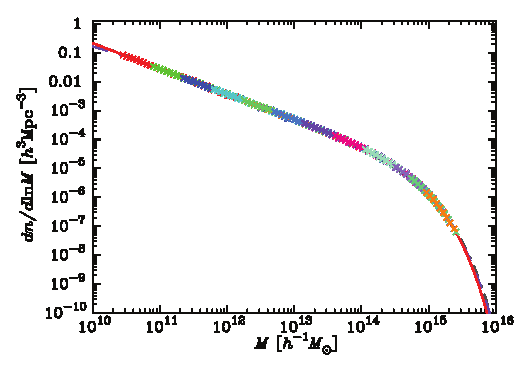
\includegraphics[width=\linewidth]{early_universe/warren_2006_mass_function.eps}
	\caption[Concentration upturn for high mass halos at high $z$]{\footnotesize The dark matter halo mass function, as measured from sixteen $1024^{3}$ particle simulations of the $\Lambda$CDM Universe.  \citep{2006ApJ...646..881W}}
	\label{fig:mass_function--warren_mass_function}
\end{figure}




%~~~~~~~~~~~~~~~~~~~~~~~~~~~~~~~~~~~~~~~~~~~~~~~~~~~~~~~~~~~~~~~~~~~~~~~~~~~~~~~
\subsection{Density and Concentration}
\label{subsec:early_universe--dark_matter_halos--density}
%~~~~~~~~~~~~~~~~~~~~~~~~~~~~~~~~~~~~~~~~~~~~~~~~~~~~~~~~~~~~~~~~~~~~~~~~~~~~~~~


The halo density profile is a measure of the spherically-averaged dark matter density as a function of radius.  For numerical halos in \nbody\ simulations, the density profile is typically computed by dividing the member particles into logarithmically-spaced bins from the virial radius inward towards the center, summing the mass of the particles in each bin, and dividing by the volume of the shell to find the density.

DM halos almost universally display a characteristic shape in their density profiles.  This shape is most often parameterized with the Navarro-Frenk-White (NFW) profile \citep{1996ApJ...462..563N}:
\begin{equation} \label{eq:nfw_profile}
	\rho(r) = \frac{ \rho_{0} }{ \frac{ r }{ R_{s}} \left( 1 + \frac{r}{R_{s}} \right)^{2} },
\end{equation}
where $\rho_{0}$ is the characteristic density and $R_{s}$ is the scale radius where the inner $\sim r^{-1}$ profile transitions to the outer $\sim r^{-3}$ profile.

Halo concentration $c$ provides a single-parameter quantization of the density profile.  For the NFW profile, concentration is defined as $c \equiv R_{\mathrm{vir}} / R_{s}$, where $R_{\mathrm{vir}}$ is the halo virial radius.  Generally, at low redshift, low mass halos are more dense than high mass halos \citep{1997ApJ...490..493N}, and concentration decreases with redshift and increases in dense environments \citep{2001MNRAS.321..559B}.  \citet{2007MNRAS.381.1450N} additionally find that concentration decreases with halo mass.  Various additional studies have explored concentration's dependence on characteristics of the power spectrum \citep{2001ApJ...554..114E}, cosmological model \citep{2008MNRAS.391.1940M}, redshift \citep{2008MNRAS.387..536G, 2011MNRAS.411..584M}, and halo merger and mass accretion histories \citep{2002ApJ...568...52W, 2003MNRAS.339...12Z, 2009ApJ...707..354Z}.  For halos at high redshift, \citet{2011ApJ...740..102K} find that concentration reverses and increases with mass for high mass halos, while \citet{2012MNRAS.423.3018P} find that concentration's dependence on mass and redshift is more complicated and is better described through $\sigma(M,z)$, the rms fluctuation amplitude of the linear density field.

Concentration may be estimated from a halo's virial mass $\Mvir$ and maximum circular velocity
\begin{equation}
	\Vcirc = \left. \sqrt{\frac{GM(<r)}{r}} \right|_{\mathrm{\max}}.
\end{equation}
Following \citet{2011ApJ...740..102K}, we outline this relationship for $z = 0$ and as a function of redshift.  The relation between the virial mass and maximum circular velocity may be given as \citep{2001ApJ...554..903K}:
\begin{equation}
	\Vcirc = \left[ G \frac{f(x_{\max})}{f(c)} \frac{c}{x_{\max}} \hat{\rho}^{1/3} \right]^{1/2} \Mvir^{1/3},
\end{equation}
\begin{equation}
	\hat{\rho} = \frac{\Mvir}{\Rvir^{3}} = \frac{4 \pi}{3} \Delta_{\mathrm{vir}} \rho_{c} \Omega_{\mathrm{M}},
\end{equation}
\begin{equation}
	f(x) = \ln(1 + x) - \frac{x}{1 + x},
\end{equation}
where $x = r / R_{s}$, $x_{\max} = 2.15$, $\Delta_{\mathrm{vir}}$ is the overdensity limit that defines the virial radius, $\rho_{c}$ is the critical density, and $\Omega_{\mathrm{M}}$ is the matter contribution to the average density of the universe.  At $z = 0$, $\Delta_{\mathrm{vir}} = 360$ and $\Omega_{\mathrm{M}} = 0.27$, which yields
\begin{equation}
	\Vcirc(\Mvir) = \frac{6.72 \times 10^{-3} \Mvir^{1/3} \sqrt{c}}{\sqrt{\ln(1 + c) - c / (1 + c)}}
\end{equation}
for $\Mvir$ in units of $h^{-1} \Msun$ and $\Vcirc$ in units of km s$^{-1}$.  \citet{2011ApJ...740..102K} find that at $z = 0$, this yields the approximation
\begin{equation}
	c(\Mvir) = 9.60 \left( \frac{\Mvir}{10^{12} h^{-1} \Msun} \right)^{-0.075}
\end{equation}
for distinct halos and
\begin{equation}
	c(M_{\mathrm{sub}}) = 12 \left( \frac{M_{\mathrm{sub}}}{10^{12} h^{-1} \Msun} \right)^{-0.12}
\end{equation}
for subhalos.  Figure~\ref{fig:concentration--klypin_concentration_upturn} plots concentration as a function of virial mass from $z = 0$ to $z = 5$.  The dotted lines are given by
\begin{equation} \label{eq:concentration_mass_upturn}
	c(\Mvir,z) = c_{0}(z) \left( \frac{\Mvir}{10^{12} h^{-1} \Msun} \right)^{-0.075} \times \left[ 1 + \left( \frac{\Mvir}{M_{0}(z)} \right)^{0.26} \right],
\end{equation}
where $c_{0}(z)$ and $M_{0}(z)$ are free parameters for each $z$.  Concentration displays a decreasing trend with mass at low redshift.  At higher redshift, however, concentration flattens out and reverses its trend, increasing with mass for the most massive halos.

\begin{figure}[ht]
	\centering
	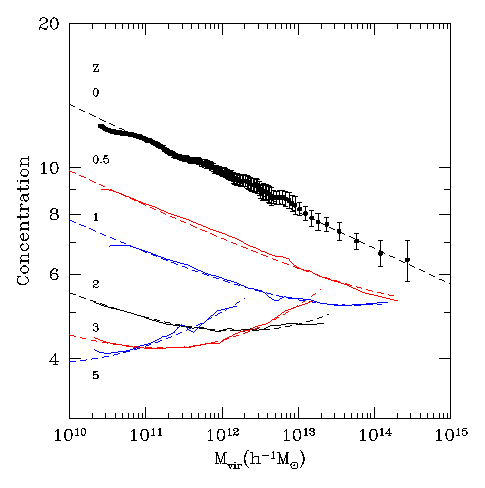
\includegraphics[width=\linewidth]{early_universe/klypin_2011_concentration_upturn.eps}
	\caption[Concentration upturn for high mass halos at high $z$]{\footnotesize Concentration as a function of virial mass for distinct halos from $z = 0$ to $z = 5$.  Symbols and solid curves are numerical results, while the dashed curves are analytical fits (Equation~\ref{eq:concentration_mass_upturn}).  Concentration decreases with increasing mass except for high-mass halos at high redshift, for which the concentration flattens and increases with mass.  \citep{2011ApJ...740..102K}}
	\label{fig:concentration--klypin_concentration_upturn}
\end{figure}

Figure~\ref{fig:concentration--klypin_concentration_z_dependence} plots concentration as a function of redshift for two representative halo masses.  For a given fixed halo mass, concentration decreases with redshift for low redshift, then increases again with redshift at high redshift.  The black curves are given by
\begin{equation} \label{eq:concentration_redshift_upturn}
	c(\Mvir, z) = c(\Mvir, 0) [\delta^{4/3}(z) + \kappa(\delta^{-1}(z) - 1)],
\end{equation}
where $\delta(z)$ is the linear growth factor of fluctuations normalized to $\delta(0) = 1$ and $\kappa$ is a free parameter.  For the masses shown in the figure, $\kappa = 0.084$ for $M = 3 \times 10^{11} h^{-1} \Msun$ and $\kappa = 0.135$ for $M = 3 \times 10^{12} h^{-1} \Msun$.

\begin{figure}[ht]
	\centering
	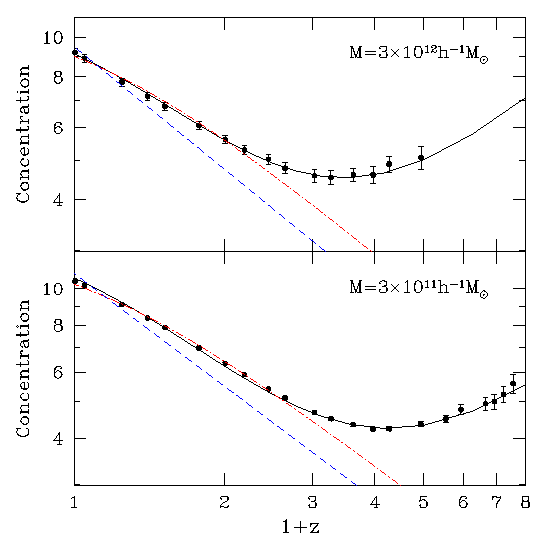
\includegraphics[width=\linewidth]{early_universe/klypin_2011_concentration_z_dependence.eps}
	\caption[Evolution of concentration with redshift for two halo masses]{\footnotesize Concentration as a function of redshift for two representative halo masses.  Black dots are simulation results.  The dashed blue curves show the power law $c \propto (1 + z)^{-1}$ and the dot-dashed red curves are $c \propto \delta$.  The solid black curves are given by Equation~\ref{eq:concentration_redshift_upturn}.  Concentration initially decreases with redshift, but reverses and increases with redshift for high redshift.  Concentration for both masses reaches a minimum of $c_{\min} \approx 4-4.5$. \citep{2011ApJ...740..102K}}
	\label{fig:concentration--klypin_concentration_z_dependence}
\end{figure}

Using the same method of determining concentration from halo virial mass and maximum circular velocity, \citet{2012MNRAS.423.3018P} find that the complex mass and redshift dependence of concentration found by \citet{2011ApJ...740..102K} may be simplified to a universal U-shaped profile when viewed as a function of the linear rms fluctuation of the density field $\sigma(M,z)$.  Figure~\ref{fig:concentration--prada_c_sigma} plots $c$ as a function of $\log \sigma^{-1}$ for redshifts from $z = 0$ to $z = 6$ for halos from the Bolshoi \citep{2011ApJ...740..102K} and MultiDark \citep{2012MNRAS.423.3018P} simulations.  If we define
\begin{equation}
	x \equiv \left( \frac{\Omega_{M,0}}{\Omega_{\Lambda,0}} \right)^{1/3} a,
\end{equation}
\begin{equation}
	a \equiv (1 + z)^{-1}
\end{equation}
where $\Omega_{M,0}$ and $\Omega_{\Lambda,0}$ are the matter and cosmological constant contributions to the density of the universe at $z = 0$, then the overplotted curve is given by
\begin{equation} \label{eq:prada_universal_sigma}
	c(M,z) = B_{0}(x)C(\sigma'),
\end{equation}
\begin{equation}
	\sigma' = B_{1}(x) \sigma(M,x),
\end{equation}
\begin{equation} \label{eq:prada_universal_sigma_scaled}
	C(\sigma') = A \left[ \left( \frac{\sigma'}{b} \right)^{c} + 1 \right] \exp\left( \frac{d}{\sigma'^{2}} \right),
\end{equation}
where $A = 2.881$, $b = 1.257$, $c = 1.022$, and $d = 0.060$.  The rms density fluctuation may be approximated as
\begin{equation}
	\sigma(M,x) = D(x) \frac{16.9 y^{0.41}}{1 + 1.102 y^{0.20} + 6.22 y^{0.333}},
\end{equation}
where
\begin{equation}
	y \equiv \left[ \frac{M}{10^{12}\ h^{-1}\ \Msun} \right]^{-1},
\end{equation}
\begin{equation}
	D(x) = \frac{5}{2} \left( \frac{\Omega_{M,0}}{\Omega_{\Lambda,0}} \right)^{1/3} \frac{\sqrt{1 + x^{3}}}{x^{3/2}} \int_{0}^{x} \frac{x^{3/2} \dd x}{(1 + x^{3})^{3/2}}.
\end{equation}
The functions $B_{0}(x)$ and $B_{1}(x)$ are defined such that they equal unity at $z = 0$ for WMAP5 parameters:
\begin{equation}
	B_{0}(x) = \frac{c_{\min}(x)}{c_{\min}(1.393)},
\end{equation}
\begin{equation}
	B_{1}(x) = \frac{\sigma^{-1}_{\min}(x)}{\sigma^{-1}_{\min}(1.393)},
\end{equation}
where
\begin{equation}
	c_{\min}(x) = c_{0} + (c_{1} - c_{0}) \left[ \frac{1}{\pi} \arctan[\alpha(x - x_{0})] + \frac{1}{2} \right],
\end{equation}
\begin{equation}
	\sigma^{-1}_{\min}(x) = \sigma^{-1}_{0} + (\sigma^{-1}_{1} - \sigma^{-1}_{0}) \left[ \frac{1}{\pi} \arctan[\beta(x - x_{1})] + \frac{1}{2} \right],
\end{equation}
\begin{equation}
	c_{0} = 3.618,\ c_{1} = 5.033,\ \alpha = 6.948,\ x_{0} = 0.424,
\end{equation}
\begin{equation}
	\sigma^{-1}_{0} = 1.047,\ \sigma^{-1}_{1} = 1.646,\ \beta = 7.386,\ x_{1} = 0.526.
\end{equation}
The resulting curve closely follows the data at all redshifts from $z = 0$ to $z = 6$, with a minimum concentration of $\sim 5$ at a well-defined scale of $\sigma \sim 0.71$.  The relation may also be seen as a function of mass without rescaling to $z = 0$ by plotting Equations~\ref{eq:prada_universal_sigma}-\ref{eq:prada_universal_sigma_scaled}, as shown in Figure~\ref{fig:concentration--prada_c_M}.

\begin{figure}[ht]
	\centering
	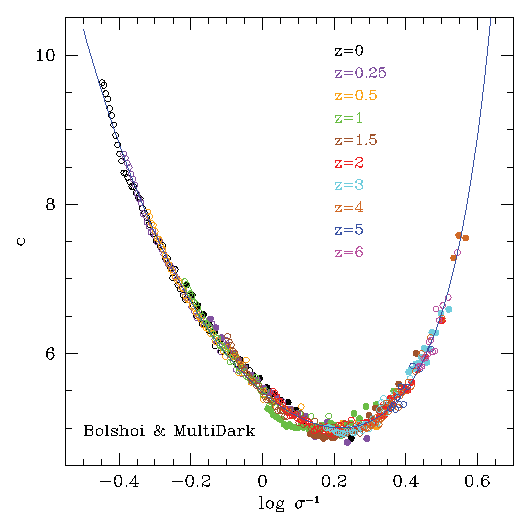
\includegraphics[width=\linewidth]{early_universe/prada_2012-c-sigma.eps}
	\caption[Halo concentration $c$ as a function of $\log \sigma^{-1}$]{\footnotesize Halo concentration $c$ as a function of $\log \sigma^{-1}$ for halos in the Bolshoi and MultiDark simulations.  The results are rescaled to $z = 0$.  The solid curve $C(\sigma')$ is given by Equation~\ref{eq:prada_universal_sigma_scaled}.  A universal minimum concentration of $\sim 5$ is seen at $\sigma \sim 0.71$.  \citep{2012MNRAS.423.3018P}}
	\label{fig:concentration--prada_c_sigma}
\end{figure}

\begin{figure}[ht]
	\centering
	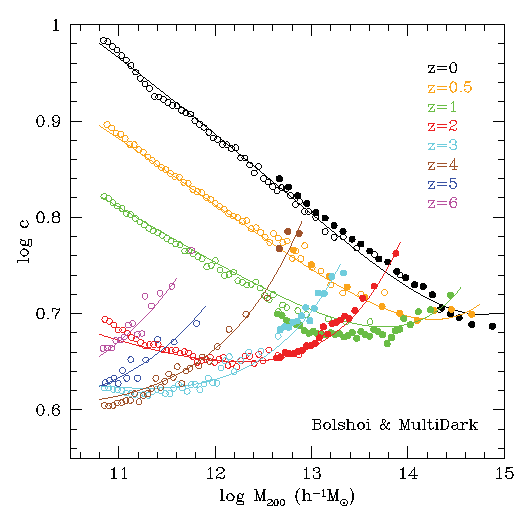
\includegraphics[width=\linewidth]{early_universe/prada_2012-c-M.eps}
	\caption[Halo concentration $c$ as a function of halo mass]{\footnotesize Halo concentration $c$ as a function of halo mass at various redshifts for halos in the Bolshoi (open circles) and MultiDark (filled circles) simulations.  The overplotted curves are given by Equations~\ref{eq:prada_universal_sigma}-\ref{eq:prada_universal_sigma_scaled}.  The analytical approximations fit the data within a few percent.  \citep{2012MNRAS.423.3018P}}
	\label{fig:concentration--prada_c_M}
\end{figure}




%~~~~~~~~~~~~~~~~~~~~~~~~~~~~~~~~~~~~~~~~~~~~~~~~~~~~~~~~~~~~~~~~~~~~~~~~~~~~~~~
\subsection{Halos as Hosts to Baryonic Processes}
\label{subsec:early_universe--baryonic_processes}
%~~~~~~~~~~~~~~~~~~~~~~~~~~~~~~~~~~~~~~~~~~~~~~~~~~~~~~~~~~~~~~~~~~~~~~~~~~~~~~~


Early-forming dark matter halos provide an incubator for the baryonic processes that transform the surrounding space and allow galaxies to form.  Initial gas accretion can lead to the formation of the first Pop-III stars \citep{1986MNRAS.221...53C, 1997ApJ...474....1T, 2000ApJ...540...39A, 2002Sci...295...93A}, which, upon their death, can collapse into the seeds for supermassive black holes (SMBHs) \citep{2001ApJ...551L..27M, 2003MNRAS.340..647I, 2009ApJ...701L.133A, 2012ApJ...754...34J} or enrich the surrounding medium with metals through supernovae \citep{2002ApJ...567..532H, 2003ApJ...591..288H}.  The radiation from these early quasars \citep{1987ApJ...321L.107S, 1999ApJ...514..648M, 2001AJ....122.2833F}, Pop-III stars \citep{1997ApJ...486..581G, 2003ApJ...584..621V, 2006ApJ...639..621A}, and proto-galaxy stellar populations \citep{2012ApJ...752L...5B, 2012MNRAS.423..862K} all play a key role in contributing to the re-ionizing the universe by around $z = 6$ \citep{2001PhR...349..125B}.  Additionally, halo mergers can drastically increase the temperature of halo gas through shock heating, increasing X-ray luminosity \citep{2009MNRAS.397..190S}, and contribute to the unbinding of gas to form the warm-hot intergalactic medium \citep{2008SSRv..134..141B, 2010MNRAS.405L..31S, 2012MNRAS.425.2974T}.




